\chapter{姿勢推定}
\thispagestyle{empty}
\label{chap3}
\minitoc

%\newcommand{\argmax}{\mathop{\rm arg~max}\limits}
%\newcommand{\argmin}{\mathop{\rm arg~min}\limits}

\newpage
%%%%%%%%%%%%%%%%%%%%%%%%%%%%%%%%%%%%%%%%%%%%%%%%%%%%%%%%%%%%%%%%%%%%%%%%%%%%%%%
%==============================================================================
% 3.1
%==============================================================================
\section{はじめに}

本章では,カメラの姿勢を推定する手法について述べる.

3.2節にて,手法の概要について述べる.

3.3節にて,球面勾配ベクトルの計算方法を述べる.

3.4節にて,単位球面勾配ベクトルの集合への3平面の当てはめについて説明する.

\newpage
%==============================================================================
% 3.2
%==============================================================================
\section{姿勢推定の概要}

姿勢推定では,推定する画像1枚からカメラの姿勢を推定する.
ここで,ワールド座標系を$z$軸回りに$\psi$ deg,$y$軸回りに$\theta$ deg,$x$軸回りに$\phi$ degずつ順に回転させた座標系がカメラ座標系$x_{\rm{sph}}y_{\rm{sph}}z_{\rm{sph}}$の向きと一致するような$\bm{O}=[\phi, \theta, \psi]^{\mathrm{T}}$をカメラの姿勢と定義する.
また,$z$軸回りに$\psi$ deg,$y$軸回りに$\theta$ deg,$x$軸回りに$\phi$ degずつ順に回転させる回転行列を$\bm{R}_{\rm{ori}}$とする.
ワールド座標系とカメラ座標系を図\ref{fig:orientation}に示す.
\\

\begin{figure}[b]
 \begin{center}
 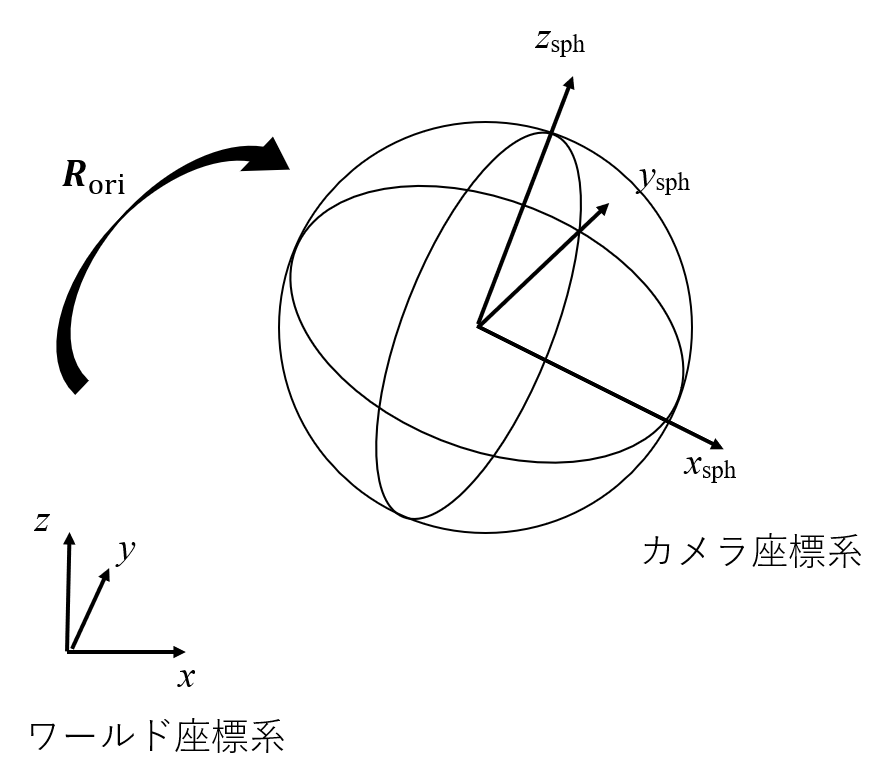
\includegraphics[width=0.6\columnwidth]{./chap3/fig/orientation.png}
 \caption{ワールド座標系とカメラ座標系}
 \label{fig:orientation}
 \end{center}
\end{figure}

対象物が球上に投影される全天球カメラモデルにおいて,図\ref{fig:spherical_gradient}に示すように,青い実線で示す環境中の直線は,大円の一部として青い破線で示すように投影される.
この青い破線上において赤い矢印で示す球面勾配は,元の直線と直交する向きとなる.
すなわち,この球面勾配ベクトルは,元の直線方向を法線ベクトルとする,図に青く示す平面上に存在する.
環境中の他の直線についても同様に,直線が投影された線上の点における球面勾配ベクトルは,もともとの直線の方向を法線ベクトルとする平面上に存在する.
本研究では,対象とする環境が人工物である屋内環境であるため,マンハッタンワールド仮説\mbox{\cite{Coughlan2001}}を適用することが可能である.
すなわち,環境中の直線はワールド座標系の$x$軸,$y$軸,$z$軸のいずれかの方向であるため,直線が投影された線上の各点における球面勾配ベクトルは,それぞれの軸方向を法線ベクトルとする平面上に分布する.
また,大きさが1となるように正規化した単位球面勾配ベクトルは,それぞれの軸方向を法線ベクトルとする大円上に分布する.
カメラ座標系$x_{\rm{sph}}y_{\rm{sph}}z_{\rm{sph}}$を回転行列$\bm{R}^{-1}_{\rm{ori}}$で回転した座標系$x'_{\rm{sph}}y'_{\rm{sph}}z'_{\rm{sph}}$は,ワールド座標系$xyz$と同じ向きとなるため,単位球面勾配ベクトルの分布は図\ref{fig:three_directions}のように表すことができる.
ここで,赤,緑,青の点はそれぞれ$x$軸,$y$軸,$z$軸方向の直線が投影された線上の点における球面勾配ベクトルを正規化した単位球面勾配ベクトルの終点である.
\\

\begin{figure}[tb]
 \begin{center}
 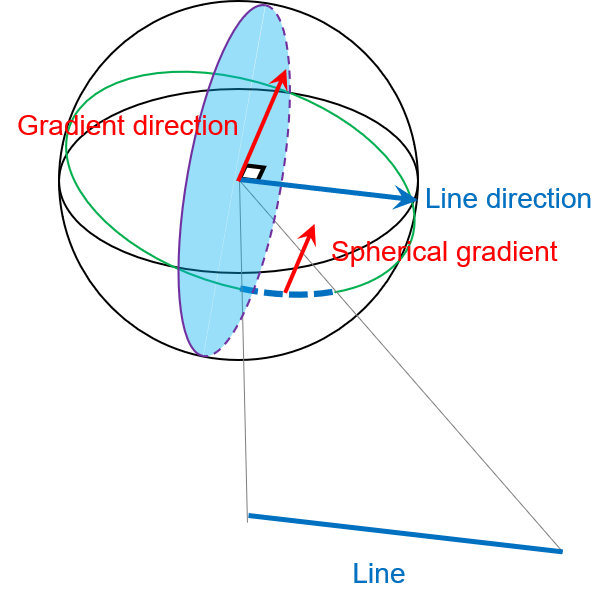
\includegraphics[width=0.55\columnwidth]{./chap3/fig/spherical_gradient.png}
 \caption{球面勾配ベクトル}
 \label{fig:spherical_gradient}
 \end{center}
\end{figure}

\begin{figure}[tb]
 \begin{center}
 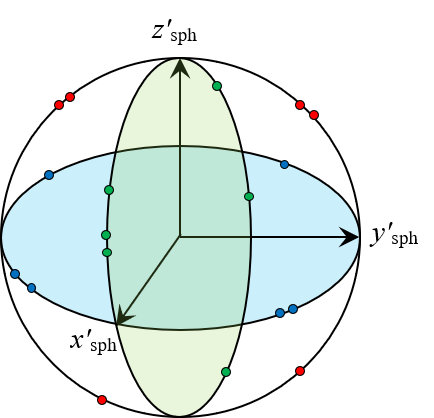
\includegraphics[width=0.45\columnwidth]{./chap3/fig/three_directions.png}
 \vspace{5mm}
 \caption{単位球面勾配ベクトルの分布}
 \label{fig:three_directions}
 \end{center}
\end{figure}

姿勢推定の流れを図\ref{fig:flow3}に示す.
まず,推定する画像から球面勾配ベクトルを計算し,単位球面勾配ベクトルの集合を得る.
次に,得られた単位球面勾配ベクトルの集合に,互いに直交する3方向を法線ベクトルとする3平面を当てはめることで,姿勢$\bm{O}$の推定値$\bm{O}^*=[\phi^*, \theta^*, \psi^*]^{\mathrm{T}}$を得る.
ここで,互いに直交する3方向の初期値としてカメラ座標系$x_{\rm{sph}}y_{\rm{sph}}z_{\rm{sph}}$の3軸を用い,単位球面勾配ベクトルの集合に当てはまるように回転させたときの回転行列が$\bm{R}^{-1}_{\rm{ori}}$,このときの3方向が,座標系$x'_{\rm{sph}}y'_{\rm{sph}}z'_{\rm{sph}}$の3軸である.


\begin{figure}[b]
 \begin{center}
 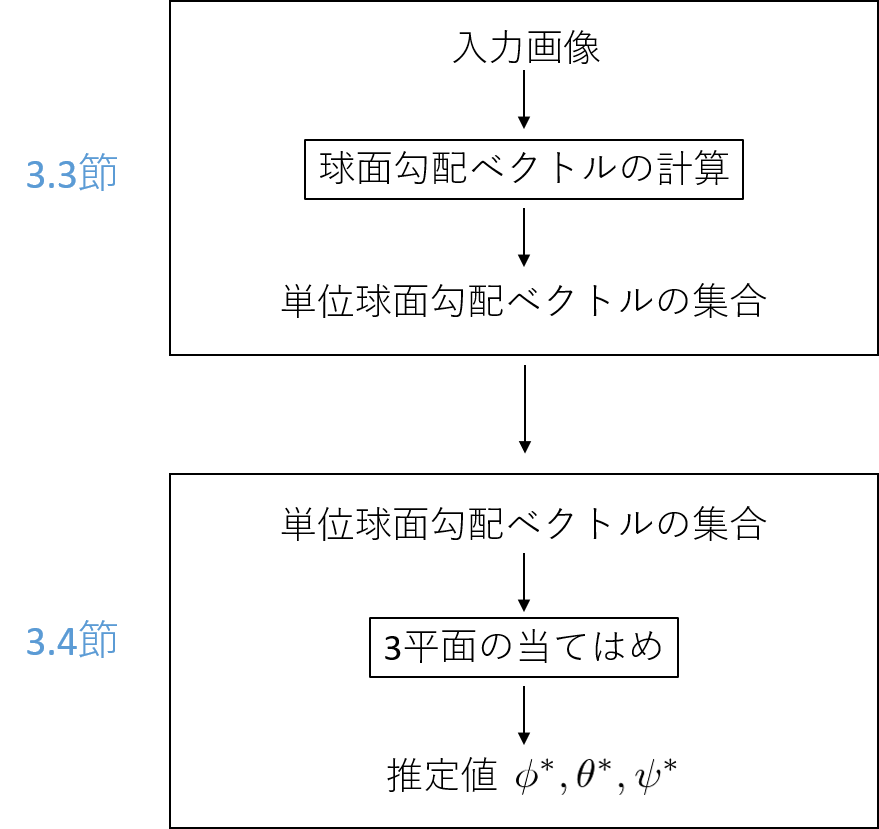
\includegraphics[width=0.6\columnwidth]{./chap3/fig/flow3.png}
 \vspace{5mm}
 \caption{姿勢推定の流れ}
 \label{fig:flow3}
 \end{center}
\end{figure}

\clearpage
%==============================================================================
% 3.3
%==============================================================================
\section{球面勾配ベクトルの計算}

球面勾配ベクトルは,全天球カメラ画像の表現方法の一つである正距円筒画像内の2次元の勾配ベクトルを変換することによって求められる.
投影される球面上の座標$\bf{\hat{x}}$$=[x,y,z]^{\mathrm{T}}$と,正距円筒画像内の座標$\bf{u}$$=[u,v]^{\mathrm{T}}$の対応関係は,画像の高さ$h$を用いて,式~(\ref{spheq})により表される.

\begin{equation}
\begin{aligned}
& x=\sin\big(\frac{\pi u}{h}\big)\sin\big(\frac{\pi v}{h}\big), \\[2.5pt]
& y=-\cos\big(\frac{\pi u}{h}\big)\sin\big(\frac{\pi v}{h}\big), \\[2.5pt]
& z=\cos\big(\frac{\pi v}{h}\big).
\end{aligned}
\label{spheq}
\end{equation}

ここで,図\ref{fig:stretch}で青と赤の線で比較されるように,球面を長方形に引き延ばすことで得られる正距円筒画像は,上端と下端に向かうほど引き延ばされる量が大きくなり,映像の歪みが大きくなる.
引き延ばされる量は式~(\ref{stretch})によって計算される$r$を用いて,$1/r$に比例して大きくなる.

\begin{equation}
\begin{aligned}
 r & =\sqrt{1-z^2} \\[2pt]
   & = \sqrt{1-\cos^2\big(\frac{\pi v}{h}\big)}.
\end{aligned}
\label{stretch}
\end{equation}

\begin{figure}[b]
 \begin{center}
 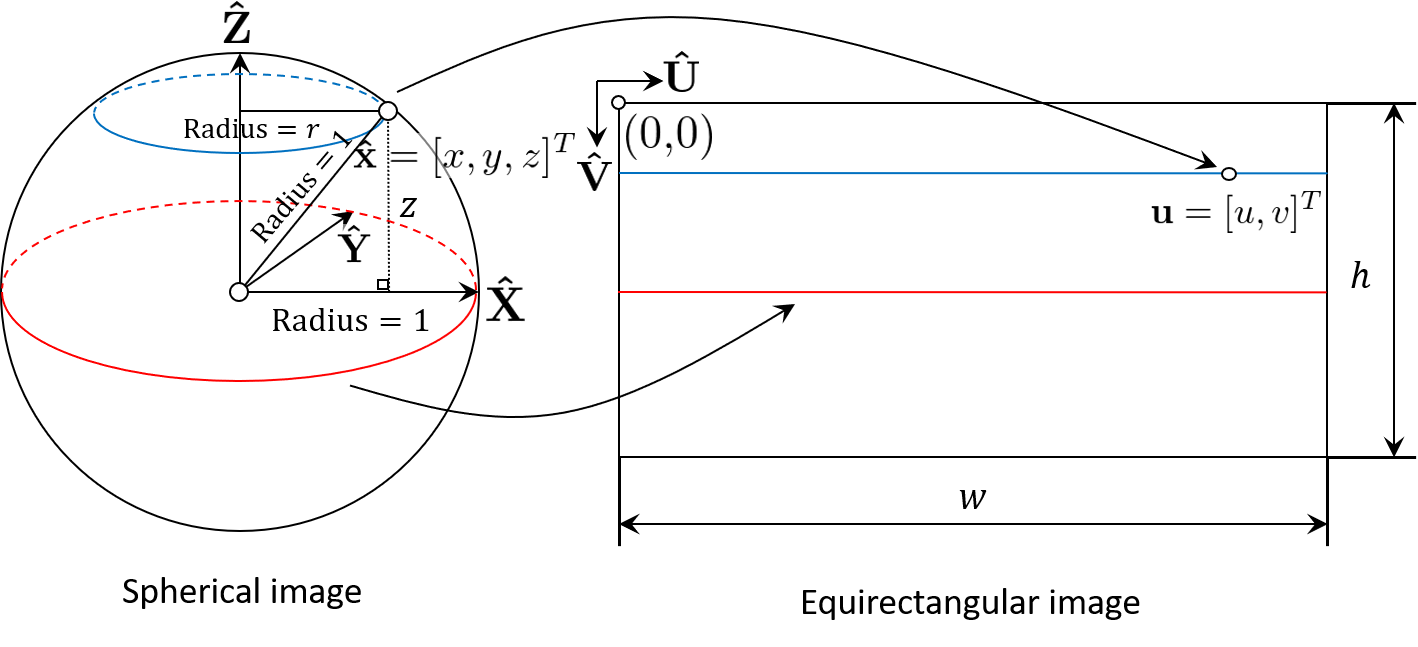
\includegraphics[width=0.9\columnwidth]{./chap3/fig/stretch.png}
 \vspace{3mm}
 \caption{球面からの正距円筒画像への展開}
 \label{fig:stretch}
 \end{center}
\end{figure}

\newpage

歪みが大きい領域では勾配を精度よく計算することができないため,入力画像における球面上の座標$\bf{\hat{x}}$における画素値を,式~(\ref{rotationeq})で表される,$x$軸回りに-90 deg回転させる行列$\bm{R}_{-90}$を用いて回転させた座標$\bm{R}_{-90}$$\bf{\hat{x}}$に移動させる.
これにより,図\ref{fig:calcgrad}に赤く示す,入力画像における上下それぞれ4分の1ずつの領域を画像中部に移動させる.
この赤い領域については,上記の回転によって得られた画像を用いることで,歪みの影響を減らして精度よく勾配を計算する.
\begin{equation}
  \bm{R}_{-90} = \left(
    \begin{array}{ccc}
      1 & 0 & 0 \\
      0 & 0 & 1 \\
      0 & -1 & 0
    \end{array}
  \right).
\label{rotationeq}
\end{equation}

\begin{figure}[b]
 \begin{center}
 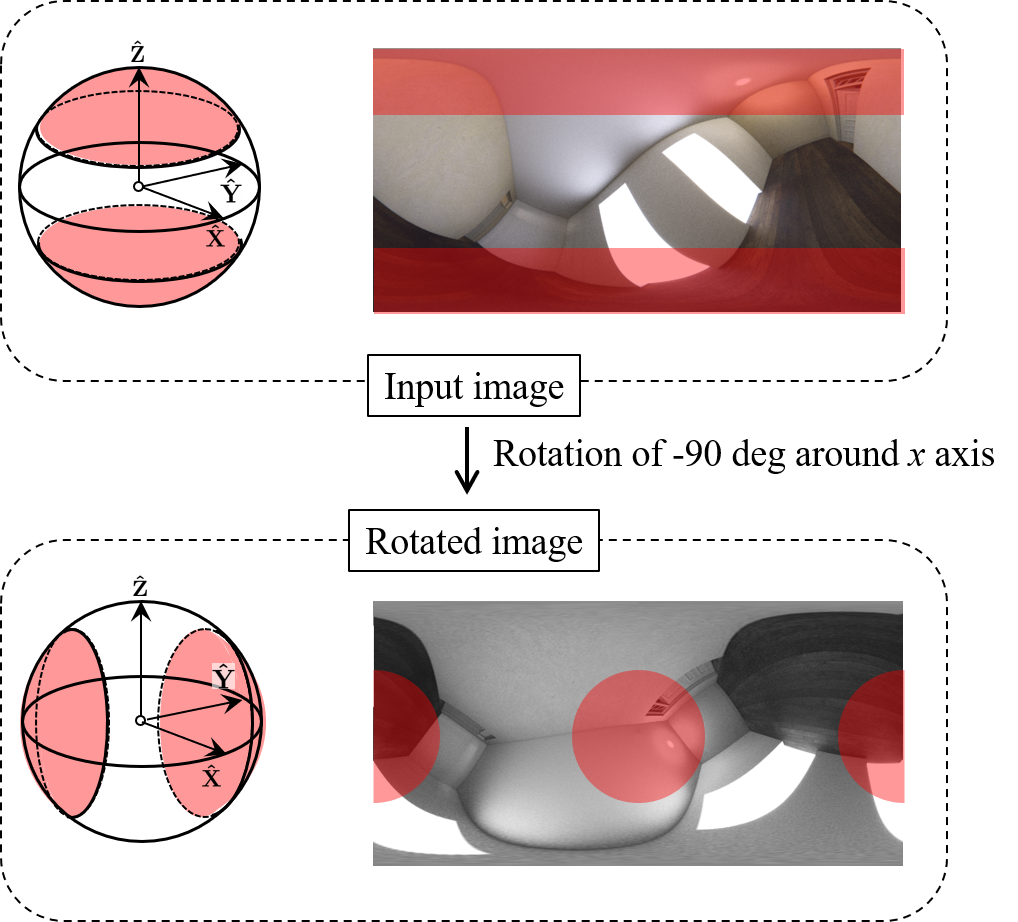
\includegraphics[width=0.65\columnwidth]{./chap3/fig/calcgrad.png}
 \vspace{3mm}
 \caption{画像の回転}
 \label{fig:calcgrad}
 \end{center}
\end{figure}

入力画像と回転された画像それぞれに対して,Cannyのエッジ検出\mbox{\cite{Canny1986}}を用いてエッジ点$(u, v)$とエッジ点における2次元の勾配ベクトル$(du, dv)$を検出する.
正距円筒画像においてエッジは通常歪んだ線となるが,Cannyのエッジ検出の計算に用いられる注目画素の周囲$3\times3$の領域においてはエッジを直線に近似することができるため,中心差分を用いた勾配の計算により,図\ref{fig:edge_detection}に示すようにエッジを検出できる.
エッジ画像において赤く示す点が入力画像から計算したエッジ点を,青く示す点が回転された画像から計算したエッジ点を表す.
画像の幅を$w$ pixelとすると,球面勾配ベクトル $(dx, dy, dz)$は以下の式を用いて図\ref{fig:conversion}に示すように求められる.

\begin{equation}
dx = \frac{2\pi}{w}\left(\cos\frac{2\pi u}{w}\sin\frac{2\pi v}{w}du+\sin\frac{2\pi u}{w}\cos\frac{2\pi v}{w}dv\right),
\end{equation}
\begin{equation}
dy= \frac{2\pi}{w}\left(\sin\frac{2\pi u}{w}\sin\frac{2\pi v}{w}du-\cos\frac{2\pi u}{w}\cos\frac{2\pi v}{w}dv\right),
\end{equation}
\begin{equation}
dz= -\frac{2\pi}{w}\sin\frac{2\pi u}{w}dv.
\end{equation}

\setlength
\subfigcapskip{-0.6ex}
\begin{figure}[h]
	%\vspace{-5mm}
	\begin{center}
		\subfigure[入力画像]{
		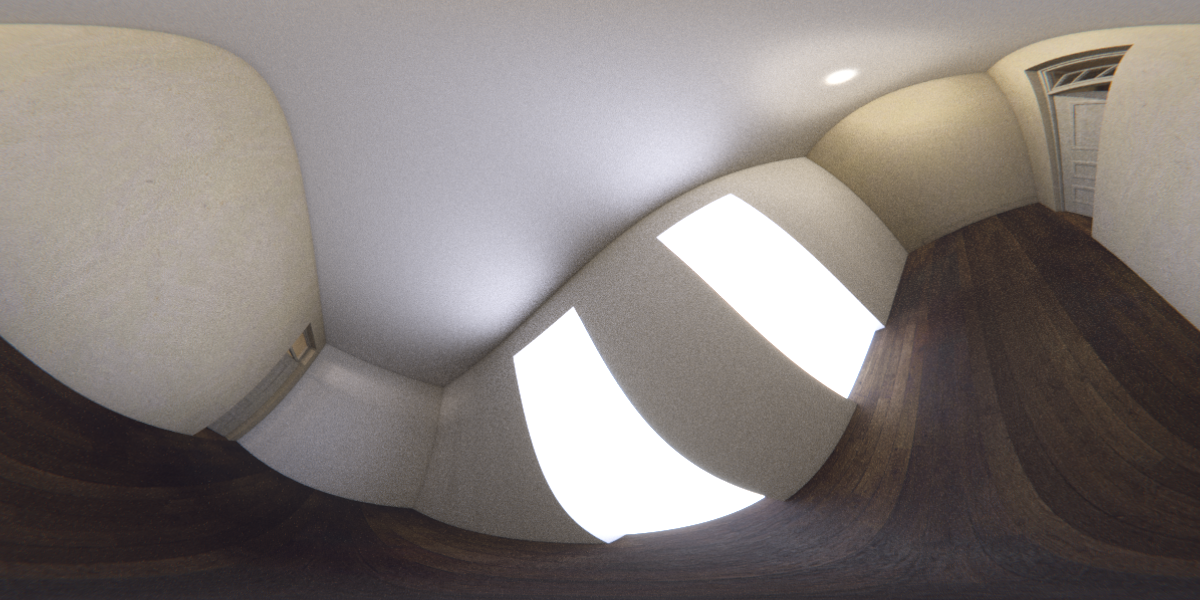
\includegraphics[clip,width=0.45\columnwidth]{./chap3/fig/frame00106.png}}\\
		\vspace{-5mm}
		\subfigure[エッジ画像]{
		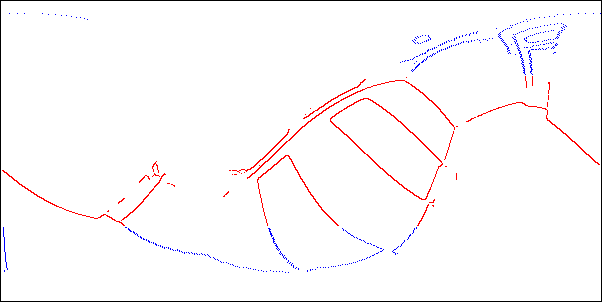
\includegraphics[clip,width=0.45\columnwidth]{./chap3/fig/edge_106.png}}
		\vspace{-3mm}
	\caption{エッジ検出の例}
	\label{fig:edge_detection}
	\end{center}
	%\vspace{-7mm}
\end{figure}

\begin{figure}[b]
 \begin{center}
 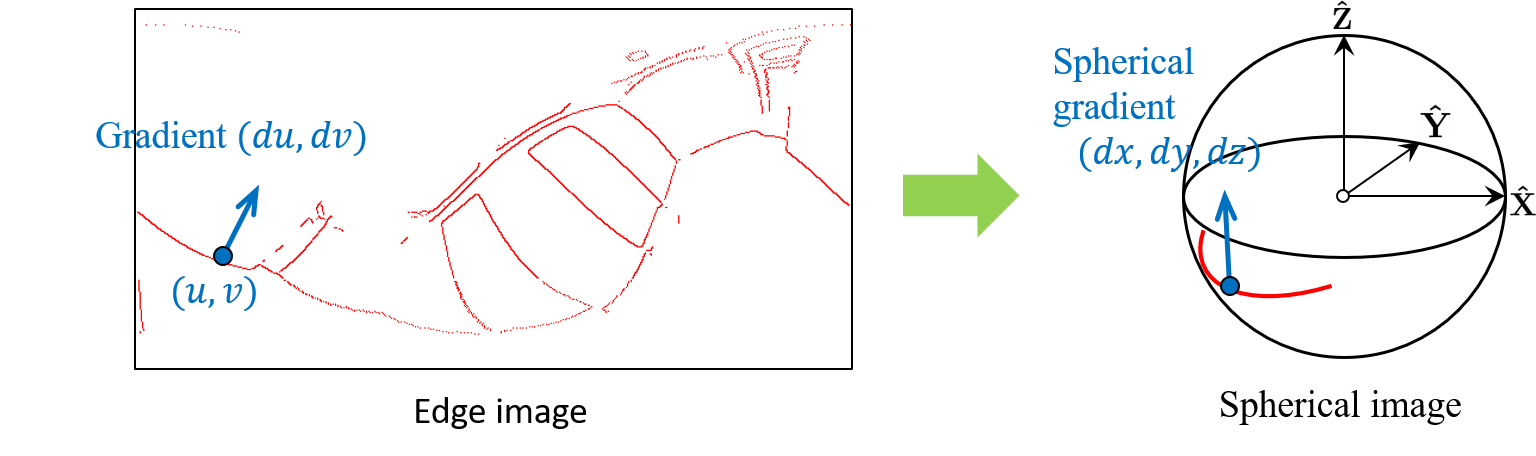
\includegraphics[width=0.85\columnwidth]{./chap3/fig/conversion.png}
 \vspace{0mm}
 \caption{画像勾配から球面勾配への変換}
 \label{fig:conversion}
 \end{center}
\end{figure}

\newpage

回転された画像から計算した球面勾配ベクトルを$x$軸回りに90度回転させて元の座標系に戻すことで,画像全体のエッジ点における球面勾配ベクトルの集合を得ることができる.
最後に,得られた球面勾配ベクトルを,単位球面上に分布するように正規化する.
単位球面勾配ベクトルの集合の例を図\ref{fig:distribution}に示す.
青,赤,緑の大円が直交する3平面を表し,青,赤,緑の点がそれぞれの平面に属するエッジ点における単位球面勾配ベクトルの終点,黒の点がどの平面にも属しないoutlierを表す.
各勾配ベクトルがどの平面に属するかについての判別方法については次節で述べる.
図\ref{fig:distribution}(a)が,回転させた画像を用いず歪みを考慮しない場合の集合で,図\ref{fig:distribution}(b)が,歪みを考慮した場合の集合である.
歪みの考慮によりoutlierが減っており,精度よく勾配を計算できていることが確認できる.


\setlength
\subfigcapskip{-0.6ex}
\begin{figure}[tb]
	%\vspace{-10mm}
	\begin{center}
		\subfigure[歪みの考慮なし]{
		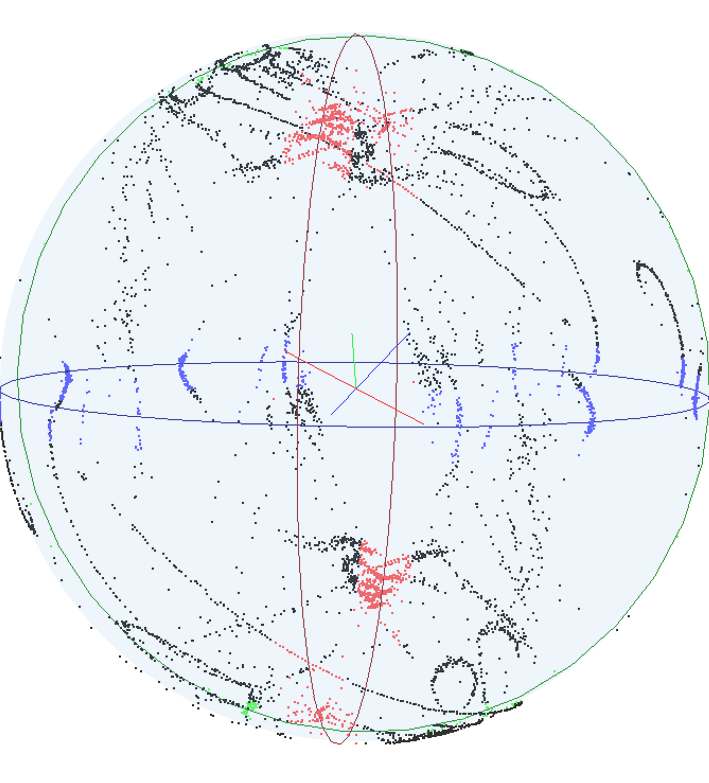
\includegraphics[clip,width=0.5\columnwidth]{./chap3/fig/gradient1.png}
		\vspace{10mm}}\\
		%\vspace{-5mm}
		\subfigure[歪みの考慮あり]{
		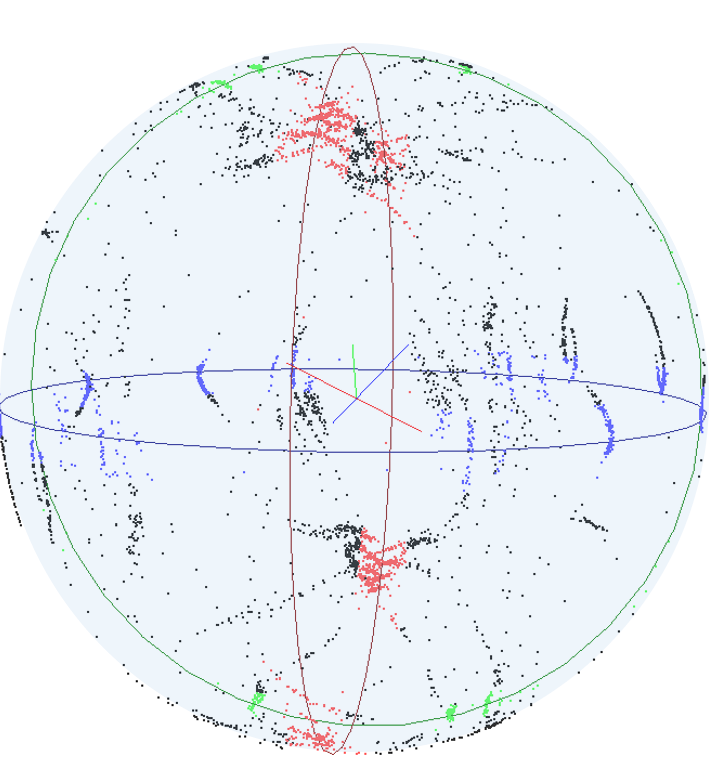
\includegraphics[clip,width=0.5\columnwidth]{./chap3/fig/gradient2.png}}
	\caption{単位球面勾配ベクトルの分布の例}
	\label{fig:distribution}
	\end{center}
	%\vspace{-7mm}
\end{figure}

\clearpage
%==============================================================================
% 3.4
%==============================================================================
\section{単位球面勾配ベクトルの集合への3平面の当てはめ}

前節で求めた計$n$個の単位球面勾配ベクトルを$\bm{v}_k\ (k=1, 2,..., n)$,ワールド座標系の3つの軸方向を $\bm{p}_i\ (i=1, 2, 3)$とすると, $\bm{v}_k$とそれぞれの平面の距離$d_{i,k}$は,それらが成す角度を用いて以下のように計算できる.
\begin{equation}
   d_{i,k} = \sin^{-1}(\bm{v}_k\cdot \bm{R}_{\rm{ori}}\bm{p}_i),
\end{equation}

各勾配ベクトル $\bm{v}_k$に対して,これらの3つの距離のうち最も近いものを$d_{k}$とする.
\begin{equation}
   d_k = \min\left(d_{1,k},\ d_{2,k},\ d_{3,k}\right).
\end{equation}

Levenberg-Marquardt法\cite{Marquardt1963}による最適化によって,すべての勾配ベクトルについての距離$d_k$の二乗和を最小とするようなパラメータ$(\phi^*,\theta^*,\psi^*)$を求める.
 
\begin{equation}
(\phi^*,\theta^*,\psi^*)=\argmin_{\phi,\theta,\psi} \sum_{k=1}^nd_k^2.
\label{eq:optim2}
\end{equation}

ここで,上記の最適化によって得られるパラメータは,ワールド座標系の各軸方向を,カメラ座標系の各軸方向のうち最も近い方向にあるものまでの回転を表すものである.
2.2節で述べた前提により,ワールド座標系の$z$軸方向はカメラ座標系の$z$軸方向が最も近い方向となるが,残りの2軸方向については図\ref{fig:four_orientation}に示すように,4通りの組み合わせが考えられる.
そこで,これら4つの候補を用いて,それぞれに対して次章で述べる位置推定を行い,3次元モデルから抽出した直線特徴と最もよくマッチングしたものを姿勢の推定値とする.

\begin{figure}[b]
 \begin{center}
 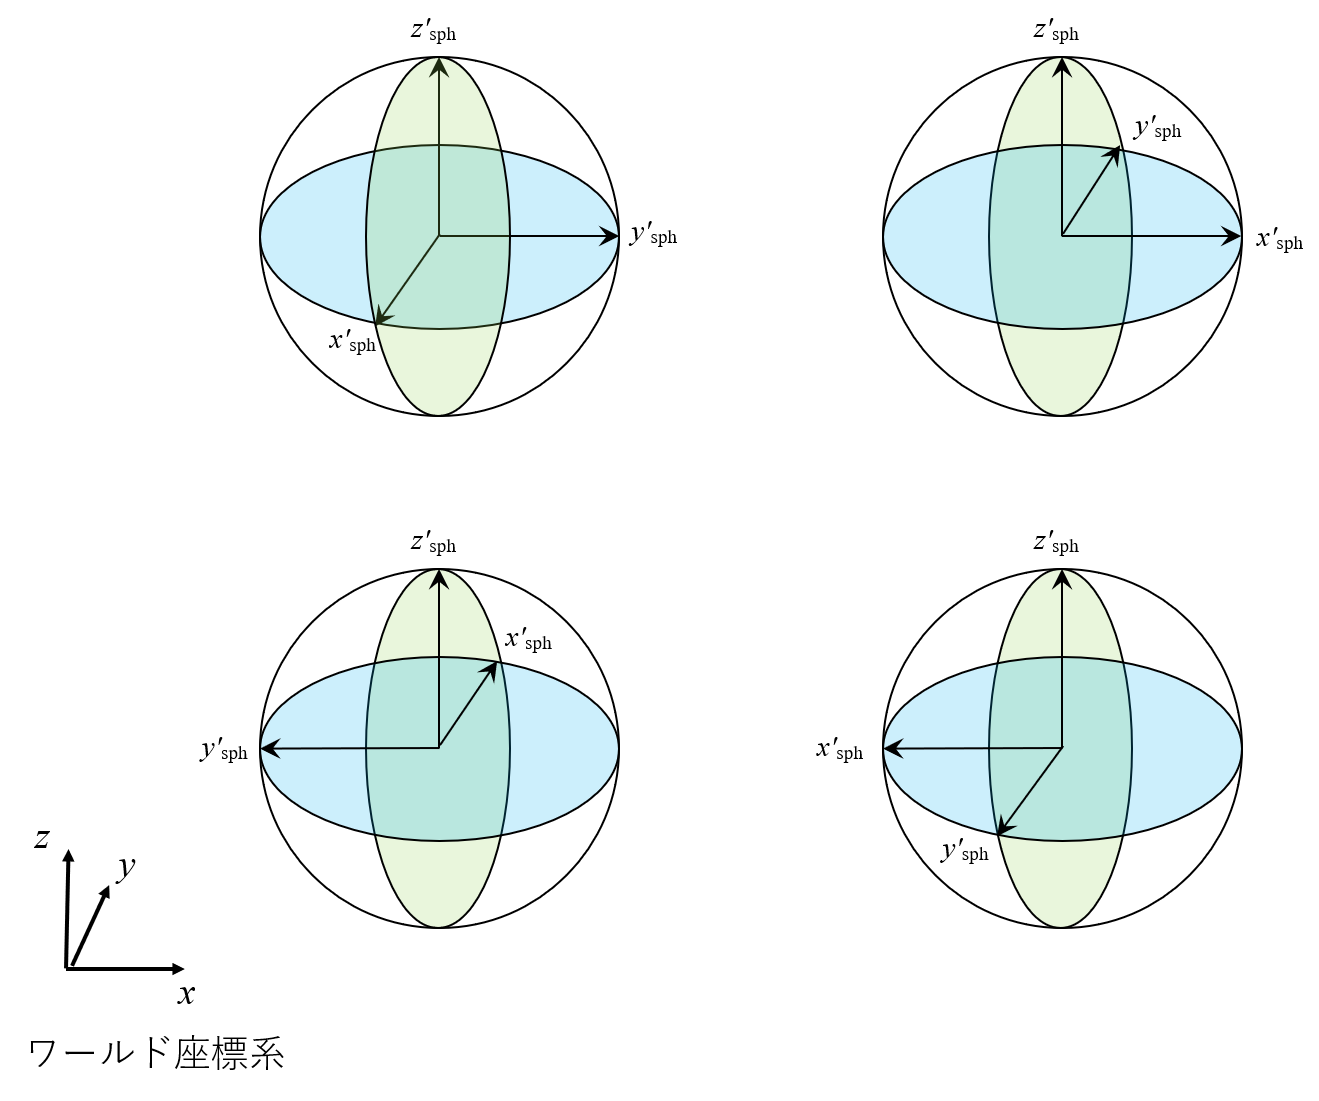
\includegraphics[width=0.9\columnwidth]{./chap3/fig/four_orientation.png}
 \vspace{0mm}
 \caption{各軸方向の4通りの組み合わせ}
 \label{fig:four_orientation}
 \end{center}
\end{figure}

\clearpage
%==============================================================================
% 3.6
%==============================================================================
\section{おわりに}

本章では,姿勢推定手法について説明した.

まず3.2節にて,姿勢推定の概要について述べた.

3.3節にて,球面勾配ベクトルの計算方法を述べた.

3.4節にて,単位球面勾配ベクトルの集合への3平面の当てはめについて説明した.

次章では,位置推定の手法について詳しく説明する.


%%%%%%%%%%%%%%%%%%%%%%%%%%%%%%%%%%%%%%%%%%%%%%%%%%%%%%%%%%%%%%%%%%%%%%%%%%%%%%%
%%% Local Variables:
%%% mode: katex
%%% TeX-master: "../thesis"
%%% End:
